\documentclass{article}

\usepackage{geometry}
\usepackage{makecell}
\usepackage{array}
\usepackage{multicol}
\usepackage{setspace}
\usepackage{changepage}
\usepackage{booktabs}
\usepackage[explicit]{titlesec}
\usepackage{hyperref}
\usepackage{graphicx}
\usepackage{cprotect}
\usepackage{float}
\usepackage{wrapfig}
\newcolumntype{?}{!{\vrule width 1pt}}
\newcommand{\paragraphlb}[1]{\paragraph{#1}\mbox{}\\}
\renewcommand{\contentsname}{Inhaltsverzeichnis:}
\renewcommand\theadalign{tl}
\setstretch{1.10}
\setlength{\parindent}{0pt}

\titleformat{\section}
  {\normalfont\Large\bfseries}{\thesection}{1em}{\hyperlink{sec-\thesection}{#1}
\addtocontents{toc}{\protect\hypertarget{sec-\thesection}{}}}
\titleformat{name=\section,numberless}
  {\normalfont\Large\bfseries}{}{0pt}{#1}

\titleformat{\subsection}
  {\normalfont\large\bfseries}{\thesubsection}{1em}{\hyperlink{subsec-\thesubsection}{#1}
\addtocontents{toc}{\protect\hypertarget{subsec-\thesubsection}{}}}
\titleformat{name=\subsection,numberless}
  {\normalfont\large\bfseries}{\thesubsection}{0pt}{#1}

\hypersetup{
    colorlinks,
    citecolor=black,
    filecolor=black,
    linkcolor=black,
    urlcolor=black
}

\geometry{top=12mm, left=1cm, right=2cm}
\title{\vspace{-1cm}Webtechnologien und Usability}
\author{Andreas Hofer}

\begin{document}
	\maketitle
	\tableofcontents
	\newpage
	\section{Einführung}
	Das Internet ist ein System verbundener Netzwerk, welche mit Protokollen interagieren. Diesen Protokollen liegt das Packet Switching zugrunde. Das Internet ist jedoch nicht das World Wide Web (WWW), welches nur eine Anwendung ist die auf einem Hypermediasystem basiert. Das WWW enthält Resourcen und Links, welche diese miteinander verbinden und baut auf 3 Grundkonzepten auf:
	\begin{itemize}
		\item{Hypertext Transfer Protocol (HTTP)}
		\begin{itemize}
			\item{Erlaubt Zugriff auf Ressourcen eines Webservers. Das geschieht mittels Anfragen und Antworten (Requests und Responses)}
		\end{itemize}
		\item{Uniform Resource Identifier (URI)}
		\begin{itemize}
			\item{Erlaubt die eindeutige Identifizierung von Resourcen (Web Adressen)}
			\item{In der Vergangenheit gab es mehrere verschiedene Protokolle, welche durch das URI ersetzt wurden.}
		\end{itemize}
		\item{Hypertext Markup Language (HTML)}
		\begin{itemize}
			\item{Textbasierte Markupsprache (Auszeichnungssprache)}
			\item{Markup erlaubt die Gliederung und Formatierung von Daten, welche danach von einem Webbrowser interpretiert wird.}
			\item{Hyperlinks erlauben Verweise zwischen HTML Dokumenten}
		\end{itemize}
	\end{itemize}
	\subsection{Uniform Resource Identifier (URI)}
	URI erlaubt nicht nur die Verwendung von HTTP Adressen, sondern auch anderen wie mailto (Zum Versenden von E-Mails) oder FTP. \\
	URIs haben stets eine spezielle Formattierung: \verb|<scheme>:[authority]<path>[?<query>][#<fragment>]|. \\
	Das scheme identifiziert den Typ der Ressource wie zum Beispiel HTTP oder mailto. \\
	Die authority gibt die Domäne an, welche angesprochen wird. Eine solche Domäne kann eine Portnummer sein. (Siehe 1/NET1/5.7 [TODO Netzwerk]) \\
	Der path dient zur Identifizierung einer Ressource und kann aus mehreren Teilen bestehen, welche durch  Schrägstriche "/" getrennt sind.\\
	Die query ist Zusatzinformation, welche an den Server übergeben werden soll und folgt immer einem Fragezeichen "?". Mehrere queries können durch das Ampersand getrennt werden "\&". \\
	Das fragment gibt an, welche Teile auf der angefragten Seite gesucht werden.
	\subsubsection{URL und URN}
	Der Uniform Resource Locator (URL) und Uniform Resource Name (URN) sind zwei Teile der URI. Obwohl beide unter URI Verwendung finden, wird URL oft als synonym zu URI gesehen, da eine URN nur über die URL angesprochen werden kann. Die URN beschreibt den Namen der Resource und wird in dem Schema \texttt{urn:1234-5678-9012} angegeben. Diese finden unter anderem für Bücher Verwendung um die ISBN (International Standard Book Number) zu beschreiben.
	\section{Hypertext Markup Language (HTML)}
	HTML ist die grundlegende Resource, welche alle Websites verwenden. HTML gibt die Struktur, sowie die Formatierung für eine Seite an. Ein HTML Dokument kann zusätzlich zu der Struktur auch Javascript (JS) zur dynamischen Veränderung der Website, sowie Cascading Style Sheets (CSS) zum Styling der Element enthalten. \\
	HTML ist momentan in der fünften Version mit HTML 5. Der Name HTML besteht aus zwei Teilen: Hypertext sowie Markup Language. \\
	Hypertext ist ein Netzwerk an Dokumenten, welche wie ein Netz untereinander verbunden sind. Eine Markup Language ist eine Formatierungsstrategie, in welcher spezifische Teile mit Kennern ausgezeichnet werden können, welche danach in einer bestimmten Weise interpretiert werden. \\
	Eine Website besteht in der Regel aus mehr als einem einzelnen HTML Dokument sondern einer ganzen Sammlung welche jeweils untereinander verlinken und so die Erscheinung einer dynamischen Website geben können. Der Einstiegspunkt einer Website wird \texttt{index.html} genannt und dient als Anfangspunkt für die Navigation. \\
	\subsection{Elemente}
	Ein HTML Dokument besteht stets aus Elementen, welche die Struktur des Dokuments angeben. In diesen Elementen befinden sind eine oder mehrere HTML Attribute, welche jeweils ausgezeichnet werden. \\
	HTML Elemente besitzen in der Regel stets einen Start- und einen End-Tag, welche normalerweise mit größer- und kleiner gleich Zeichen ausgzeichnet werden: \texttt{<p> This is a paragraph </p>}. Ein End-Tag wird zusätzlich mit einem Slash "/" gekennzeichnet.
	\subsubsection{inline und block}
	Ein Element innerhalb eines HTML Dokuments ist stets im \texttt{inline} oder \texttt{block} Modus. Block bedeutet, dass es stets in seiner eigenen Zeile geführt wird. Also wird ein Block Element selbst ohne einem line break \texttt{<br>} in die nächste Zeile gesetzt und das nächste Element wird wiederum in der Zeile darunter. Ein inline Element hingegen kann direkt zwischen Text eingefügt werden und verbraucht genau so viel Platz wie das Element benötigt.
	\begin{figure}[H]
	\centering
	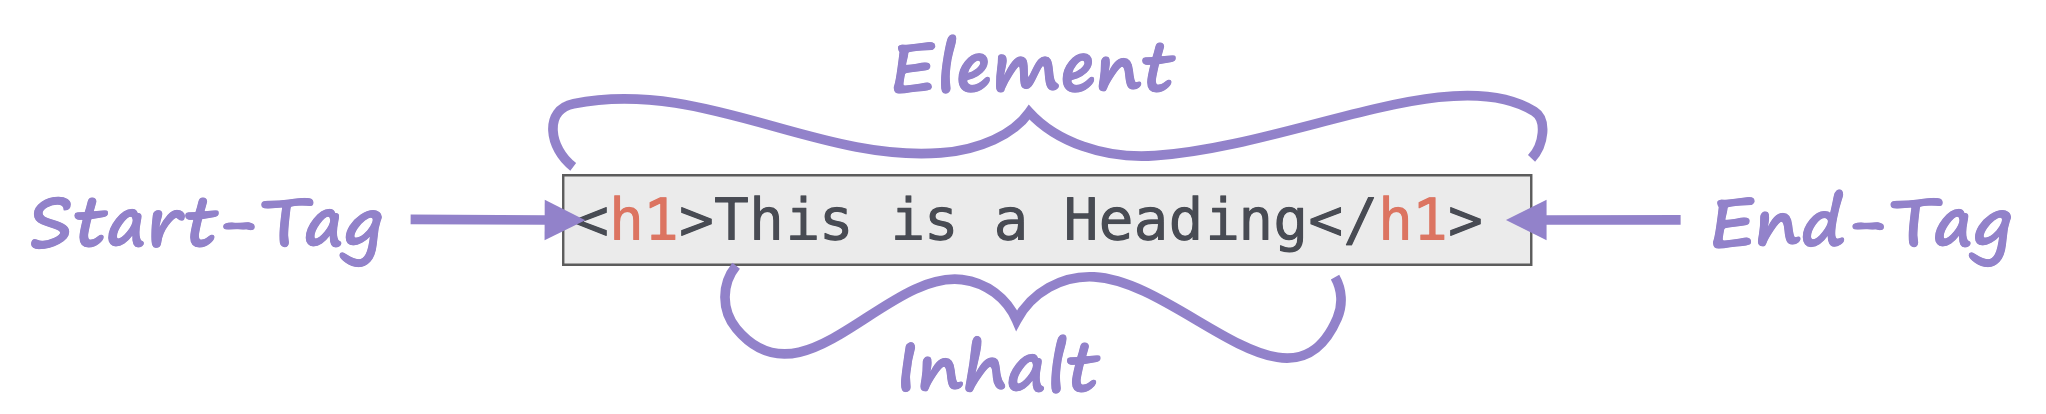
\includegraphics[scale=0.4]{Bilder/tag.png}
	\caption{Ein HTML Element sowie Start und End Tag}
	\end{figure}
	Zusätzlich gibt es auch leere Elemente, welche keinen End tag benötigen. \texttt{<br>} welches einen Line Break signalisiert, muss nicht wieder geschlossen werden. Zu beachten ist, dass Elemente sich nicht überlappen dürfen. Wenn man in einen Paragraphen begonnen hat, kann man nicht dazwischen ein anderes Element öffnen, jedoch nicht wieder schließen. \\
	HTML ist nicht case sensitive, jedoch ist es gute Form Tags stets mit Kleinbuchstaben zu schreiben. \texttt{Statt <P> eher <p>}\\
	Ein HTML Dokument beinhaltet seinen gesamten Inhalt innerhalb des \texttt{<html>} tags. Dieser Inhalt kann wiederum in zwei grobe Teile gespalten werden: Den Header, sowie den Body. Der Header gibt Metainformation über das Dokument an, während der Body der Teil ist, welcher vom User gesehen wird. \\
	Ein Kommentar kann in HTML mit \texttt{<!--} begonnen und mit \texttt{-->} wieder geschlossen werden. \\
	\texttt{<!-- I am a comment -->}
	\subsection{\texttt{<!DOCTYPE>}}
	Der doctype muss das erste Element (Noch vor \texttt{<html>}) in einem HTML Dokument sein und gibt an welche Version von HTML in dem Dokument verwendet wird.
	\subsection{Semantische Elemente}
	Semantische Elemente definieren verschiedene Teile einer Website. Semantische Elemente dienen nur zum besseren Überblick des Dokuments und können auch für Screenreader sinnvoll sein. Typische semantische Elemente sind:
	\begin{itemize}
		\item{header}
		\begin{itemize}
			\item{Der Header gibt Meta- und Zusatzinformation über die Website an}
		\end{itemize}
		\item{\texttt{<nav>}}
		\begin{itemize}
			\item{Definiert einen container für Navigationslemente innerhalb der Website}
		\end{itemize}
		\item{\texttt{<main>}}
		\begin{itemize}
			\item{Gibt Information an, welche auf dieser Seite verfügbar ist.}
			\item{Innerhalb des \texttt{<main>} Elements kann es zusätzlich weitere Elemente geben:}
			\begin{itemize}
				\item{\texttt{<section>}}
				\begin{itemize}
					\item{Definiert einen Abschnitt des Dokuments}
				\end{itemize}
				\item{\texttt{<article>}}
				\begin{itemize}
					\item{Definiert einen unabhängigen, semantisch getrennten Artikel}
				\end{itemize}
			\end{itemize}
			\item{\texttt{<aside>}}
			\begin{itemize}
				\item{Enthält Zusatzinformation, welche nicht direkt in das \texttt{<main>} Element passen.}
			\end{itemize}
			\item{\texttt{<footer>}}
			\begin{itemize}
				\item{Enthält eine Fußzeile für das Dokument}
			\end{itemize}
		\end{itemize}
	\end{itemize}
	\subsection{Nicht-Semantische Elemente}
	Es gibt auch Nicht-Semantische Elemente, welche keinen direkt zugewiesenen Zweck besitzen, das Dokument jedoch weiter strukturieren. Nicht-semantische Elemente sind:
	\begin{itemize}
		\item{\texttt{<div>}}
		\begin{itemize}
			\item{Definiert einen nicht spezifisch beschreibbaren Abschnitt des Dokuments. \texttt{<div>} ist ein Block Element, wodurch es davor und danach jeweils einen Zeileunumbruch einfügt und einen gewissen Abstand zu anderen Elementen definiert.}
		\end{itemize}
		\item{\texttt{<span>}}
		\begin{itemize}
			\item{Das inline Äquivalent zu dem \texttt{<div>}. Hiermit kann man innerhalb eines Fließtexts einen speziellen Abschnitt definieren und diesem zum Beispiel eine andere Farbe geben.}
		\end{itemize}
	\end{itemize}
	\subsection{Globale Attribute}
	Das html Element kann globale Attribute aufweisen, welche im gesamten Dokument definiert werden, diese kann man jedoch auch nur einzelne Elemente ausweisen.
	\subsubsection{lang}
	Gibt die Sprache des Elements oder des Dokuments an. Dies geschieht mittels internationaler Sprachcodes, können jedoch auch lokale Änderung angeben. (Wie \texttt{en-US}). Diese Sprachangabe kann bei Screenreadern sehr praktisch sein um sicherzustellen, dass die Software weiß in welcher Sprache sie es vorlesen sollte. \\
	\texttt{<p lang="fr"> This is a paragraph in French </p>}
	\subsubsection{id}
	Einen Element kann einer id zugewiesen werden um dieses eindeutig kennzuzeichnen. Diese id ist case sensitive, muss immer aus einem Zeichen bestehen und darf keine Leerzeichen enthalten. Jede id muss innerhalb des Dokuments eindeutig sein, also gibt es keine id scopes. Mit solchen ids kann man diese ausweisen um es über das CSS Stylesheet oder Javascript gezielt anzupassen.\\
	\texttt{<p id="start"> This is the starting paragraph </p>}
	\subsection{\texttt{<head>}}
	Der header wird mit \texttt{<head>} begonnen und mit \texttt{</head>} geschlossen. Der Header sollte sich stets zwischen dem \texttt{<html>} und dem \texttt{<body>} Tag befinden. Als Metainformationsspeicher kann man in diesem spezielle Elemente definieren:
	\begin{itemize}
		\item{\texttt{<title>}}
		\begin{itemize}
			\item{Der Titel des HTML Dokuments. Dieser wird in der Registerkarte des Browsers, sowie als Bezeichnung bei Favoriten und Suchmaschinenergebnissen angegeben.}
		\end{itemize}
		\item{\texttt{<meta>}}
		\begin{itemize}
			\item{Metainformation über das Dokument}
			\item{Beispiele für Metainformation sind die Kodierung mittels \texttt{charset} oder einer Beschreibung unter dem Titel. Ebenfalls kann man die Größe des Viewports (Der sichtbaren Größe der Website) mit meta verändern.}
			\item{\texttt{<meta charset="UTF-8"> -> Definiert die Kodierung als UTF-8}}
			\item{\texttt{<meta name="description" content="I am a description" -> Gibt die Beschreibung der Website an}}
		\end{itemize}
		\item{\texttt{<style>}}
		\begin{itemize}
			\item{Gibt Stylinginformation für das Dokument an. Dieses Element sollte in der Regel nicht verwendet werden und jegliches styling sollte in einem verlinkten CSS Dokument geschehen. Das hilft dabei den Code übersichtlicher zu machen und ermöglicht es auch ein bestimmtes Styling mehrfach zu verwenden ohne dass man es mehrmals angeben muss.}
		\end{itemize}
		\item{\texttt{<script>}}
		\begin{itemize}
			\item{Einbindung von Javascript Code innerhalb des Dokuments. Dieser Code kann verwendet werden um Berechnungen auszuführen oder das Dokument dynamisch zu verändern. Gleich wie CSS Styling sollte auch Javascript Code im Idealfall mittels eines verlinkten .js Dokuments angegeben werden.}
		\end{itemize}
		\item{\texttt{<link>}}
		\begin{itemize}
			\item{Ermöglicht das Verknüpfen von dem Dokument zu externen Ressourcen. Mit diesem Element kann ein CSS oder JS Dokument mit HTML verbunden werden.}
			\item{Man muss stets zusätzlich die Art der Relation mittels \texttt{rel} und den Typ mittels \texttt{type} angeben.}
			\item{\texttt{<link rel="stylesheet" type="text/css" href=“css/theme.css">} -> CSS Dokument vom Typ stylesheet/css wird eingebettet.}
		\end{itemize}
	\end{itemize}
	\subsection{\texttt{<body>}}
	Nach dem Headerelement folgt das \texttt{<body>} Element. Diese gibt den sichtbaren Teil des Dokuments an, weshalb Text sowie Bilder in der Regel hier angegeben werden. Der Body hat auch spezielle Elemente zur Strukturierung des Dokuments:
	\begin{itemize}
		\item{\texttt{<p>}}
		\begin{itemize}
			\item{Gibt einen eigenen HTML Absatz an. Dabei werden zusätzliche Leerzeichen automatisch vom Browser entfernt.}
		\end{itemize}
		\item{\texttt{<h[x]>}}
		\begin{itemize}
			\item{Gibt Überschriften an. Diese reichen von \texttt{h1} bis \texttt{h6}, wobei eine höhere Zahl ein niedrigeres Level angibt}
		\end{itemize}
		\item{[TODO BODY]}
	\end{itemize}
	\subsection{Validation}
	HTML verlangt zwar, dass jedes Element, das es unterstützt, auch wieder geschlossen wird, erstellt jedoch keine Fehlermeldung, sollte das nicht geschehen. Gleichzeitig rendern Browser Elemente oft problemlos auch fehlerhaft geschlossene HTML Dokumente. Während dies bei dem Darstellen jedoch keine Fehlermeldung ergibt, können Screenreader und Webcrawler diese Dokumente jedoch nur eingeschränkt verarbeiten. Aus diesem Grund existieren HTML Validator, welche ein HTML Dokument auf dessen Richtigkeit überprüft.
	\section{Responsive Web Design}
	Da heutzutage Websites nicht mehr nur auf PCs aufgerufen werden, sondern sehr viele Nutzer Smartphones oder Tablets nutzen, ist es wichtig, eine Website sowohl auf dem Desktop als auch auf einem Mobilgerät nutzbar zu machen. Hierbei gibt es andere Richtlinien als bei einer Desktopseite, da diese meist breiter als höher sind, während Mobile Browser meist höher als breiter sind. Man kann Elemente benutzen um eine Website dynamisch an diese Unterschiede anzupassen:
	\begin{itemize}
		\item{Mit \texttt{viewport}, einem \texttt{meta} Element, kann man die Breite der Website an die Breite des Browsers anpassen.}
		\begin{itemize}
			\item{\texttt{<meta name="viewport" content="width=device-width", initial-scale="1.0"> -> Gibt die sichtbare Breite als die Breite des Browserfensters an.}}
		\end{itemize}
		\item{Mit dem \texttt{width} Attribut kann man die Breite eines Elements an die Breite des Browsers binden und so die Größe des Elements dynamisch anhand der Browsergröße verändern.}
		\begin{itemize}
			\item{\verb|<img src="img_girl.jpg" style="width:100%;"> -> Das Bild hat jeweils die Breite des Browserfensters|}
		\end{itemize}
		\item{Während zuvor die Größe \texttt{width} mit 100\% angegeben wurde, was die Größe des Browserfensters angibt, kann mn alternativ auch die Größen viewport width (vw) und viewport height (vh) verwenden, da der Viewport (Der tatsächlich sichtbare Teil des Browsers eventuell kleiner ist als der Browser selbst)}
	\end{itemize}
	\subsection{Document Object Model (DOM)}
	Da Elemente in einem HTML Dokument hierarchisch angeordnet sind, kann dieser auch in einer Baumstruktur angegeben werden. Diese Struktur nennt man Document Object Model (DOM) und verbindet alle Elemente innerhalb des Dokuments beginnend mit \texttt{<html>}. Der DOM ist ein wichtiges Element um Teile des Dokuments mittels Javascript zu ändern. So kann man Knoten hinzufügen oder verändern.
	\section{Cascading Style Sheets (CSS)}
	CSS ist die Standard Sprache um Stylesheets für HTML zu definieren. Mit diesem Stylesheet kann man die visuelle Gestaltung von Inhalten definieren. Man kann zwar in einem HTML Element auch den Style definieren, jedoch sollte man jegliche solche Information in dem CSS Dokument bündeln um nicht jedes Element einzeln beschreiben zu müssen. (Separation of Concerns). \\
	CSS wird verwendet um das Styling einer Website anzugeben, da HTML in sich genommen nicht besonders schön ist und nur zur Angabe der Struktur und des Inhalts verantwortlich ist. So kann man mit CSS unter anderem die Schriftart, die Farbe oder die Größe eines Elements angeben. Man kann mittels drei Wegen CSS Styling in einem HTML Element verwenden:
	\begin{itemize}
		\item{Inline}
		\begin{itemize}
			\item{Das CSS Styling wird direkt im Tag des Elements angegeben. Sollte in der Regel nicht verwendet werden.}
		\end{itemize}
		\item{Style Block}
		\begin{itemize}
			\item{Man kann im Header des Dokuments mittel \texttt{<style>} jedoch auch einen expliziten CSS Block angeben, welcher dann als Styling im gesamten Dokument verwendet wird. Ist auch eher zu vermeiden, da man es für jedes HTML Dokument separat angeben und verändern muss.}
		\end{itemize}
		\item{Separates Dokument}
		\begin{itemize}
			\item{Das Styling wird in einem separaten \texttt{*.css} Dokument angegeben und im Header verlinkt. Dieser Weg ist in der Regel der Beste, da man CSS Stylings so in mehreren Dokumenten verwenden kann und es so nicht für jedes inkludierte Dokument angeben muss.}
		\end{itemize}
	\end{itemize}
	\subsection{Übersicht}
	\subsubsection{Syntax}
	CSS hat eine spezielle Syntax um Regeln anzugeben: \\
	\texttt{h1 \{color:purple; font-size: 12px;\}} \texttt{-> selector \{property: value\}} \\
	Zuerst wird das HTML Element das angesprochen werden soll angegeben, dann dessen Attribut und schließlich dessen Wert. Werte müssen in geschwungenen Klammern \texttt{\{\}} stehen. \\
	\subsubsection{Selektoren}
	In CSS kann man Gruppen von Elementen mittels Selektoren auswählen. Dabei gibt es mehrere Gruppen um Elemente auszuwählen:
	\begin{itemize}
		\item{Element Selector}
		\begin{itemize}
			\item{Wählt alle Elemente anhand ihres Namens aus. So kann man zum Beispielalle Paragraphen miitels \texttt{p} oder alle inline spans mittels \texttt{span} ansprechen. Falls man Elemente anhand mehr als ihres Namens ändern will, muss man IDs oder Klassen haben.}
			\item{Um ein Element anzusprechen muss man nur dessen Namen angeben.}
			\item{\texttt{p \{color: blue;\}}}
		\end{itemize}
		\item{ID Selector}
		\begin{itemize}
			\item{Verwendet das id Attribut eines Elements um es zu verändern. Dabei muss id \textit{genau einem} Element entsprechen und darf nicht als Duplikat vorkommen.}
			\item{Um ein Element mittels id anzusprechen muss man davor eine Raute schreiben: \verb|#|}
			\item{\verb|#number \{color: blue;\}|}
		\end{itemize}
		\item{Class Selector}
		\begin{itemize}
			\item{Verwendet das class Attribut um ein Element zu verändern. Class, kann, im Gegensatz zu einer id, dabei mehrere Elemente gleichzeitig ansprechen.}
			\item{Um ein Element mittels id anzusprechen muss man davor einen Punkt schreiben: \texttt{.}}
			\item{\texttt{.header \{color: blue;\}}}
			\item{Zusätzlich kann man das mit Elementen kombinieren um nur diese Elementer dieser Klasse zu verändern. Dabei muss man das Element vor den Selektor schreiben: \verb|h1.header {color: blue;}|}
		\end{itemize}
		\item{Universal Selector}
		\begin{itemize}
			\item{Spricht \textit{jedes} Element an. Man kann dieses ebenfalls mit Elementen kombinieren um alle Elemente innerhalb des Elements anzusprechen.}
			\item{\texttt{* \{color: blue;\} -> Färbt jedes Element blau ein.}}
			\item{\texttt{div * \{color: blue;\} -> Färbt alle in div enthaltenen Elemente blau ein.}}
		\end{itemize}
	\end{itemize}
	\subsubsection{Kombinatoren}
	Elemente können jedoch nicht nur alleine stehen und einzeln angesprochen werden. So kann man zwischen einzelnen Elementen Kombinatoren hinzufügen um so ein Element das in spezieller Relation zu einem anderen Element steht, anzusprechen. Diese Kombinatoren sind:
	\begin{itemize}
		\item{\texttt{ (Leerzeichen)}}
		\begin{itemize}
			\item{Spricht alle Nachfahren des Elements an}
		\end{itemize}
		\item{\texttt{>}}
		\begin{itemize}
			\item{Spricht alle direkten Kinder an. (Ein Level unter dem Element)}
		\end{itemize}
		\item{\texttt{+}}
		\begin{itemize}
			\item{Angrenzende Geschwister und Nachbarn}
		\end{itemize}
		\item{\texttt{\~}}
		\begin{itemize}
			\item{Alle nachfolgenden Geschwister}
		\end{itemize}
	\end{itemize}
	\begin{figure}
	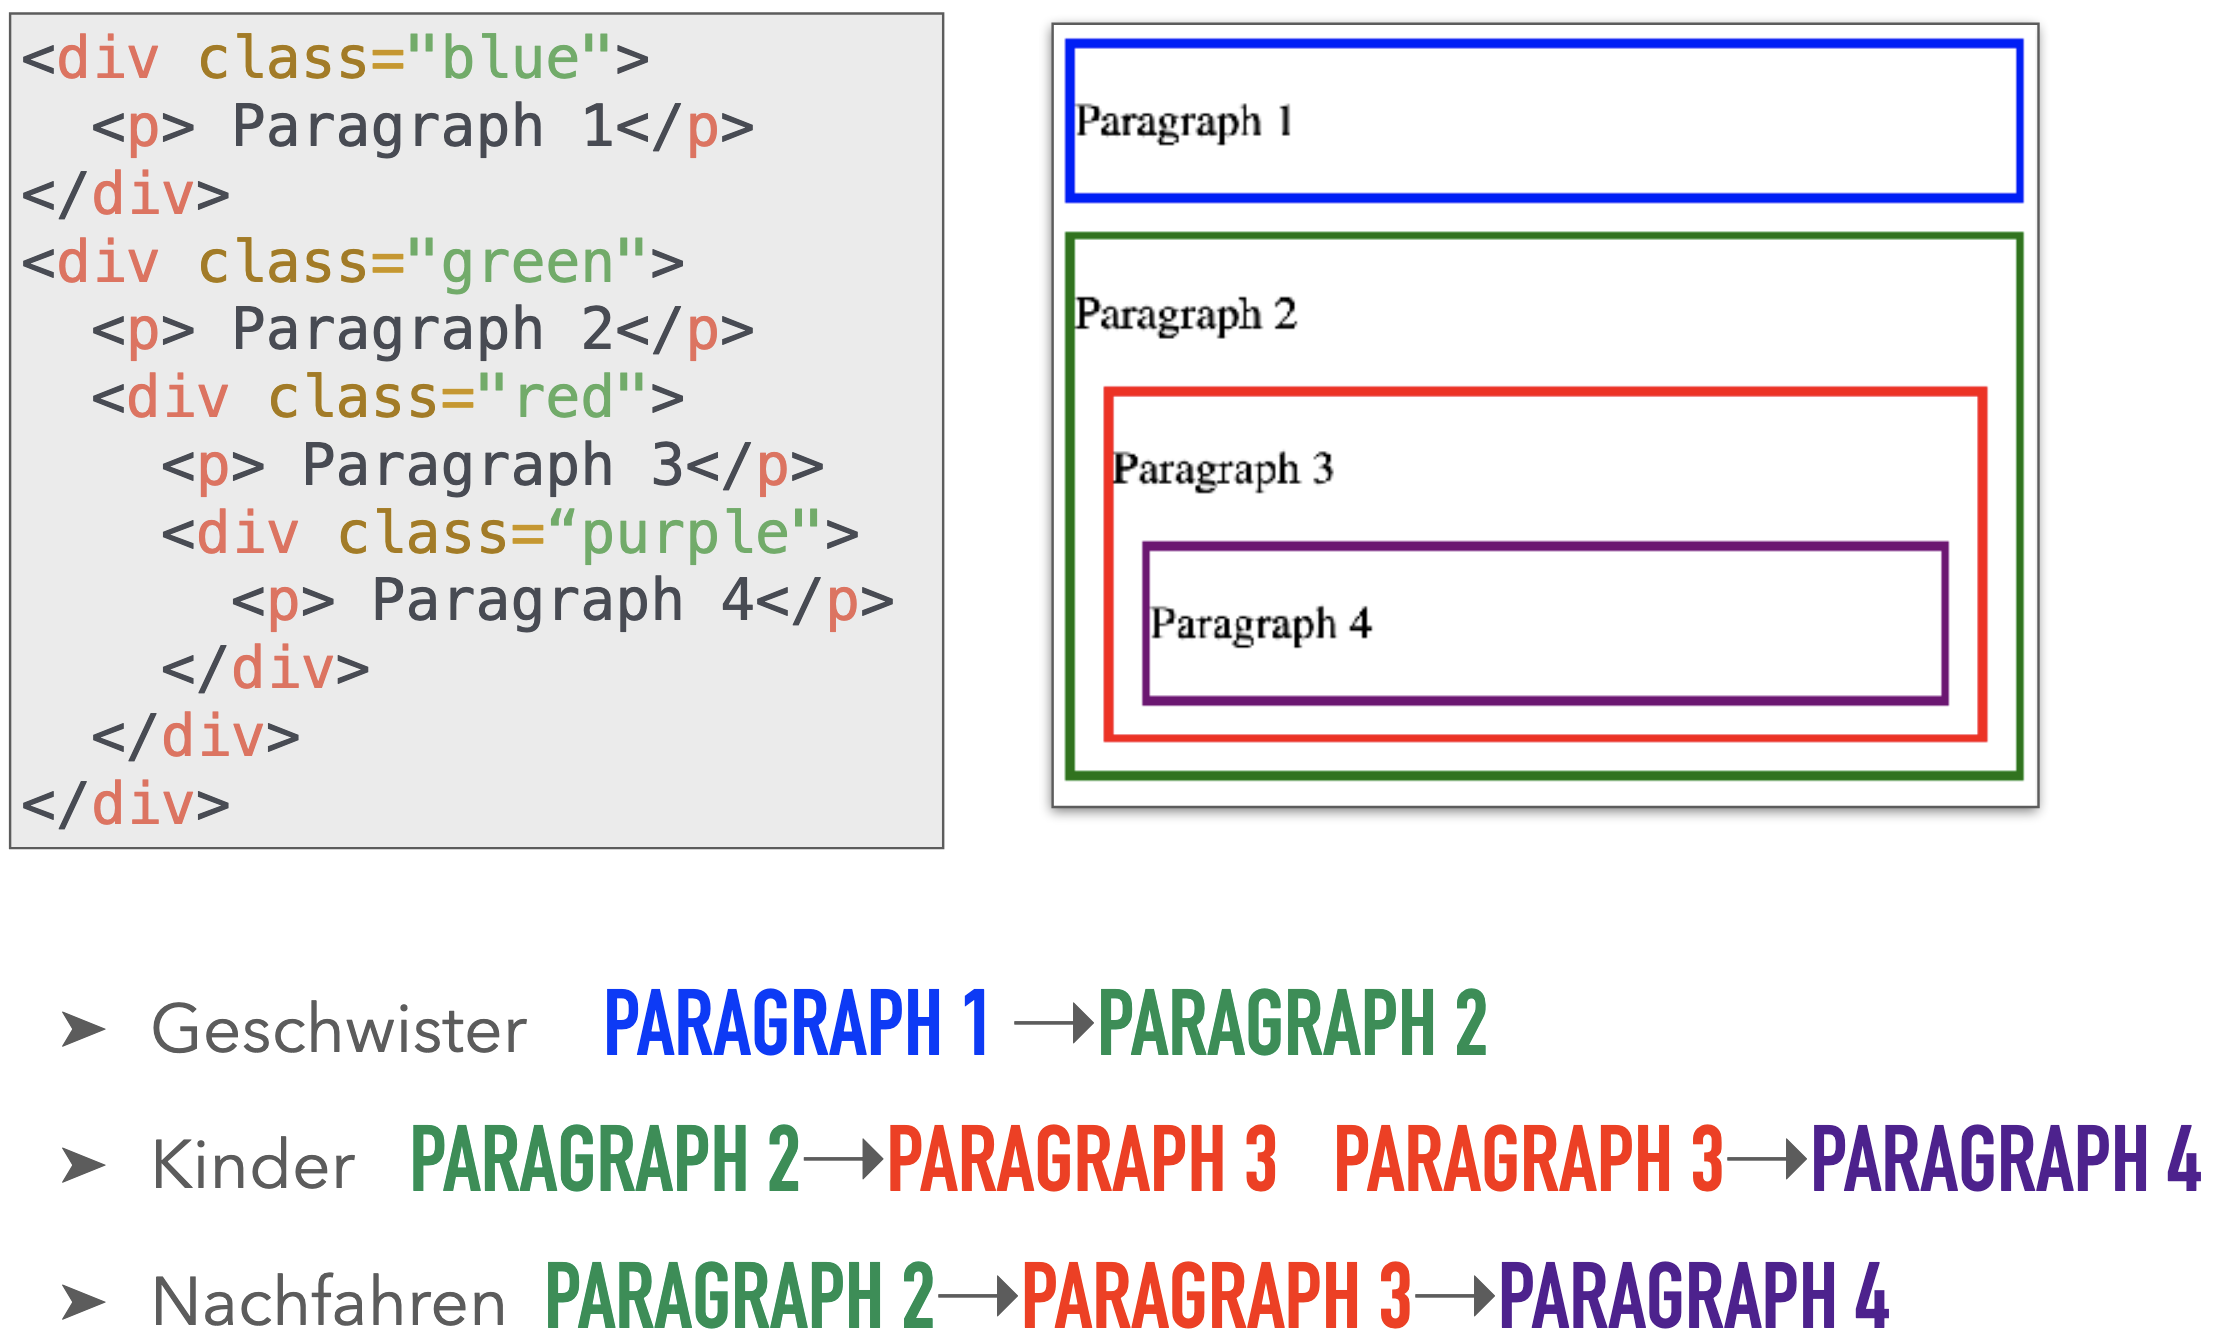
\includegraphics[scale=0.2]{Bilder/relations.png}
	\caption{Kinder, Nachbarn und Geschwister stehen in spezieller Relation}
	\end{figure}
	Hierbei muss man zuvor jedoch erst definieren, was ein Nachfahre, Kinder, Geschwister und Nachbarn sind.
	\begin{itemize}
		\item{Wenn ein Element von einem anderen Element umschlossen wird (Wenn also zum Beispiel ein Paragraph innerhalb eines divs stehen), dann ist jedes dieser Elemente ein Nachfahre.}
		\item{Ein Kind ist der Nachfahre welcher \textit{direkt} nach dem Element folgt.}
		\item{Wenn ein Element auf der selben Ebene als ein anderes Element innerhalb des selben Elements liegt, sind diese Geschwister.}
		\item{Ein Nachbar ist das Geschwisterelement, welches direkt \textit{direkt} nach dem Element folgt.}
	\end{itemize}
	\subsubsection{Cascading Order}
	Das Cascading in CSS stammt aus der Rangordnung aus welcher Elemente verändert werden. Es wurden bereits die verschiedenen Wege, wie man den Style eines Dokuments verändern kann, welche hier erneut relevant werden.
	\begin{enumerate}
		\item{Inline}
		\item{\texttt{<style>} Element im Header}
		\item{Externes CSS Stylesheet}
		\item{Standardeinstellung des Browsers}
	\end{enumerate}
	So hat ein Inlinestyle die höchste Priorität und der Browser die niedrigste. Wenn also das gleiche Attribut des gleichen Elements sowohl Inline als auch im externen Stylesheet verändert wird, wird der Style des Inline-CSS verwendet, da dieser eine höhere Priorität hat.
	\subsubsection{Specificity}
	Ein weiterer Aspekt des Cascading ist die Spezifizität von Elementen. Während zuvor dessen Quelle relevant war, ist nun wichtig, welches Attribut des Elements angesprochen wird.
	\begin{enumerate}
		\item{Style Attribut}
		\item{ID Attribut}
		\item{Class Attribut}
		\item{Element Attribut}
	\end{enumerate}
	Diese sind wiederum von der höchsten zur niedrigsten Spezifizität sortiert. Wenn also das gleiche Attribut des gleichen Elements mittels Inline Style und dem Element Selector verändert wird, hat der Inline Style eine höhere Priorität und wird anhand dessen gestyled.
	\subsubsection{Kommentare}
	Kommentare werden in CSS gleich wie in Java mit einem Slash und einem Stern eingeleitet und wiederum mit einem Stern und einem Slash beendet: \texttt{/* This is a CSS Comment */}
	\subsection{Text}
	Man kann in CSS auch spezifisch Text ansprechen. Die grundlegendste Veränderung ist dabei dessen Farbe zu ändern. CSS definiert dabei 140 Grundfarben welche mit einem Namen angesprochen werden können, diese sehen jedoch meist nicht allzu schön aus. Um diesen genauer zu verändern kann man diese auf drei Wege ansprechen:
	\begin{itemize}
		\item{RGB}
		\begin{itemize}
			\item{Besteht aus drei Werten zwischen 0 und 255 und gibt die Rot-, Grün- und Blauwerte an.}
			\item{Um eine Farbe in RGB anzugeben, muss man rgb vor die Klammer schreiben: \texttt{rgb(0, 255, 0)}}
		\end{itemize}
		\item{RGBA}
		\begin{itemize}
			\item{Funktioniert gleich wie RGB, hat jedoch zusätzlich den Alpha Channel, welcher die Deckkraft der Farbe angibt (Auch zwischen 0 und 255)}
			\item{Um eine Farbe in RGBA anzugeben, muss man rgb vor die Klammer schreiben: \texttt{rgba(0, 255, 0, 255)}}
		\end{itemize}
		\item{Hexadezimal}
		\begin{itemize}
			\item{Funktioniert gleich wie RGB, die Zahlen werden jedoch in Hexadezimalzahlen angegeben.}
			\item{Um eine Farbe als Hex anzugeben, muss man \verb|#| for die Zahlen schreiben: \verb|#00ff00|}
		\end{itemize}
		Weitere Attribute von Text sind das \texttt{text-alignment} und das \texttt{text-decoration}:
		\begin{itemize}
			\item{\texttt{text-alignment}}
			\begin{itemize}
				\item{Gibt die Bündigkeit des Textes an:}
				\begin{itemize}
					\item{Dabei sollte man jedoch beachten, dass diese Bündigkeit nur innerhalb der Grenzen des Elements geschieht und \textit{nicht} die Anordnung des Elements verändert.}
					\item{\texttt{left -> Linksbündig}}
					\item{\texttt{right -> Rechtsbündig}}
					\item{\texttt{center -> Zentriert}}
					\item{\texttt{justified -> Blocksatz}}
				\end{itemize}
			\end{itemize}
		\end{itemize}
			\item{\texttt{text-decoration}}
			\begin{itemize}
				\item{Fügt dem Text weitere Elemente hinzu:}
				\begin{itemize}
					\item{\texttt{underline -> Unterstreicht den Text}
					\item{\texttt{line-through -> Streicht den Text durch}}}
				\end{itemize}
			\end{itemize}
		\end{itemize}
		\subsubsection{Schriftart}
		Man kann auch die Schriftart des Textes ändern. Dabei bietet CSS die Möglichkeit eines Fallbacks an, welcher relevant wird, wenn der momentane Font nicht verfügbar ist. So kann man vermeiden, dass im ersten Moment, in dem die gewünschte Schriftart noch geladen wird, nicht alles in der Standardschriftart steht (Nennt man "Pop-In"). \\
		Man kann anstatt einer spezifischen Schrift jedoch auch eine Schriftfamilie (Wie \texttt{Arial}) oder, ob sie serif (Mit Verzierungen) oder sans-serif (Ohne Verzierungen) sein soll.
		\begin{verbatim}
		p {
		 font-family: "Times New Roman", serif;
		} -> Der Text des Paragraphs soll Times New Roman sein, oder die nächste serif Schrift, falls nicht möglich.
		\end{verbatim}
		\subsection{Elementgröße}
		Die Schriftgröße eines Elements kann durch eine Größenangabe verändert werden. Der offensichtlichste Weg ist dabei die Pixel der Größe direkt anzugeben. Dazu gibt man einfach die Größe mit \texttt{px} an (Ohne Leerzeichen zwischen Zahl und Einheit). Solche Größenangaben sind jedoch statisch und man kann sie nur für eine spezifische Größe anpassen. Wenn man also zum Beispiel die Größe der Elemente mittels Pixel für einen 1920x1080 16:9 Monitor anpasst, wird dieses auf einem Handybildschirm bedeutend schlechter aussehen da die Größe der Pixel sich nicht verändert und zudem ein anderes Größenverhältnis hat. Um diese Situation zu vermeiden gibt es relative Größenangaben. Zwei davon (Die \texttt{\%} und viewport) wurden bereits verwendet. Es gibt jedoch noch drei weitere gängige Größen:
		\begin{itemize}
			\item{\%}
			\begin{itemize}
				\item{Prozentuale Größe anhand des Elternelements}
			\end{itemize}
			\item{vh - Viewport Height}
			\begin{itemize}
				\item{Prozentuale Größe anhand der sichtbaren Höhe des Fensters}
			\end{itemize}
			\item{vw - Viewport Width}
			\begin{itemize}
				\item{Prozentuale Größe anhand der sichtbaren Breite des Fensters}
			\end{itemize}
			\item{em}
			\begin{itemize}
				\item{Größe abhängig von der Schriftgröße des Elternelements}
			\end{itemize}
			\item{rem}
			\begin{itemize}
				\item{Größe abhängig von der Schriftgröße des Wurzelelements}
			\end{itemize}
	\end{itemize}
	In der Regel werden em und rem nur für Schrift verwendet da man so die Schriftgrößen der Elemente automatisch anhand einer anderen Schrift anpassen kann. In der Regel ist der Viewport auch kleiner als die Gesamtgröße des Browsers, wodurch es eine genauere Angabe des Sichtbaren Feldes darstellt. Pixel sollten in der Regel nur verwendet werden, wenn sich die Größe des Elements nicht verändern soll. (Wie zum Beispiel bei einer)
	\subsection{Box Model}
	Das Box Model beschreibt die Container in welchem alle Elemente existieren. So kann man einem Element eine spezifische Position oder Hintergrundfarb zuordnen und diese gleichzeitig bündeln. Boxen haben ebenfalls Attribute um ihre Größe, Position und Ränder zu definieren.
	\begin{figure}[H]
	\centering
	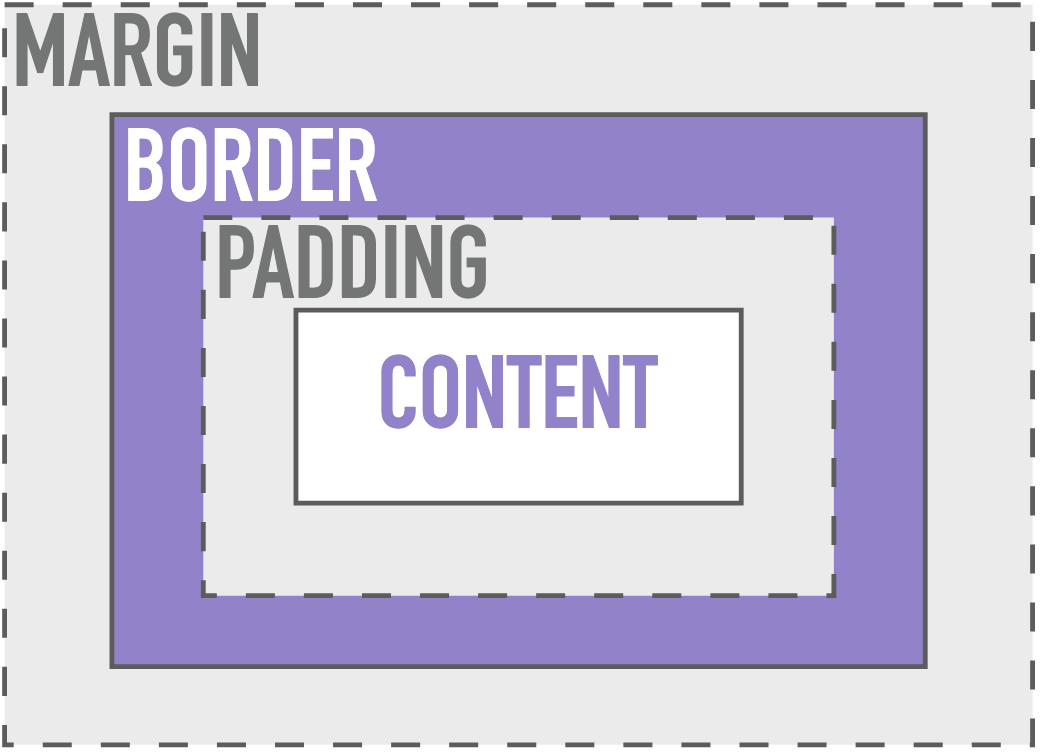
\includegraphics{Bilder/box.png}
	\caption{Die Ebenen einer Box}
	\end{figure}
	
	\subsubsection{Positionsattribute}
	[TODO Attribute]
	\subsubsection{Position}
	Bis jetzt wurden alle Elemente von dem Browser automatisch untereinander angeordnet. Manchmal will man jedoch Elemente an spezifischen Positionen haben. Das kann man auf verschiedenen Arten erreichen. Es gibt unzählige Wege um Elemente zu positionieren, hier werden jedoch nur position und die flexbox erwähnt. \\
	Mit \texttt{position} kann man angeben wie sich ein Element innerhalb der Struktur verhalten soll. Dabei unterscheidet man zwischen static, relative, static, absolute und sticky. 
	\begin{itemize}
		\item{\texttt{static}}
		\begin{itemize}
			\item{\texttt{Static} ist der Standardwert, also werden Elemente anhand ihrer Struktur automatisch angepasst. Das bedeutet jedoch auch, dass Positionsattribute darauf keinen Einfluss haben. }
		\end{itemize}
		\item{\texttt{relative}}
		\begin{itemize}
			\item{Um das zu erreichen muss man ein Element als \texttt{relative} definieren. So kann man ein Element mittels Positionsattributen anpassen, es wird jedoch nicht mehr automatisch vom Browser angepasst.}
		\end{itemize}
		\item{\texttt{fixed}}
		\begin{itemize}
			\item{Wird relativ zum Ansichtsfenster positioniert, weshalb es selbst beim scrollen an der selben Stelle bleibt.}
		\end{itemize}
		\item{\texttt{absolute}}
		\begin{itemize}
			\item{Wird relativ zum nächsten relativen (Nicht static) Elternelement angepasst. In oberster Ebene wird es relativ zum gesamten Element angepasst.}
		\end{itemize}
		\item{\texttt{sticky}}
		\begin{itemize}
			\item{Verhält sich gleich wie fixed, hat jedoch eine feste Position im Dokument und bleibt beim scrollen hängen.}
		\end{itemize}
	\end{itemize}
	\subsection{Flexbox}
	Die flexbox ist ein alternativer Weg um Elemente anzuordnen. Dabei definiert man Flexcontainer, welche Flexitems enthalten und innerhalb des Containers dynamisch angepasst werden. Sowohl der Container als auch die Items haben ihre eigenen Attribute um diese dynamische Anordnung zu beeinflussen.
	\subsubsection{Container}
	Die Attribute des Containers zeigen wie die Elemente gehandhabt werden und sich untereinander verhalten sollen.
	\begin{itemize}
		\item{\texttt{flex-direction}}
		\begin{itemize}
			\item{Gibt die Richtung an, in welche Elemente innerhalb des Containers angeordnet werden sollen. (Horizontal oder Vertikal oder Rechts/Links Oben/Unten)}
		\end{itemize}
		\item{\texttt{flex-wrap}}
		\begin{itemize}
			\item{Gibt an, ob Elemente, falls nötig, in die nächste Zeile gedrückt werden können.}
		\end{itemize}
		\item{\texttt{justify-content}}
		\begin{itemize}
			\item{Gibt an wie Elemente im Container horizontal ausgerichtet sein sollen. So kann man angeben, dass diese mittig, oder rechts oder links oder den gesamten Container (Mit Lücken dazwischen falls nötig) aufüllen sollen.}
		\end{itemize}
		\item{\texttt{align-items}}
		\begin{itemize}
			\item{Gibt an wie Elemente im Container vertikal ausgerichtet sein sollen. So kann man angeben ob Elemente oben oder unten oder in der Mitte angepasst sein sollen. Man kann auch definieren, dass Elemente den gesamten möglichen Platz vertikal ausfüllen sollen.}
		\end{itemize}
	\end{itemize}
	\section{Barrierefreiheit}
	Barrierefreiheit beschreibt die problemlose Verwendung einer Website trotz physischer Einschränkungen. So sollte man eine Website verwenden können, auch wenn man blind, gehörlos oder bewegungseingeschränkt ist.
	\subsection{Seheinschränkung}
	Bei einer Seheinschränkung sollte Text so konstrastreich wie möglich sein. Weiß/Schwarz sind sehr kontrastreiche Kombinationen. Das selbe gilt für Schwarz und Gelb. Solche kontrastreichen Kombinationen können auch bei einer Sehschwäche ausgemacht werden. Idealerweise kann man die Farbeinstellungen der Website selbst wählen, da man sich nie auf alle Gegebenheiten vorbereiten kann. Es ist ebenfalls wichtig, dass man die Skalierung von Text verändern kann um den bei Bedarf größer machen zu können.
	\subsection{Blindheit}
	Eine weitere Stufe ist komplette Blindheit. Hier geht es spezifisch um die Zugänglichkeit von Screenreadern. Dazu ist es wichtig für Bilder Alt Text einzufügen und valides HTML zu verwenden. Ein Screenreader kann ein HTML Dokument eventuell nicht richtig parsen, falls das HTML Dokument unsauber aufgebaut ist.
	\subsection{Motorische Einschränkung}
	Bei motorischen Problemen ist die Zugänglichkeit mit der Tastatur wichtig. So sollte man mittels Tab die Elemente der Website intuitiv durchlaufen können. Zusätzlich sollte man größere Knöpfe anbieten können um das auswählen einfacher zu machen.
	\subsection{Gehörlosigkeit}
	Bei Gehörlosigkeit sind Untertitel sowie Textalternativen für Videos wichtig.
	\subsection{Web Content Accesibility Guidelines (WCAG)}
	Die WCAG definiert einer Sammlung an Guidelines um das Web für alle zugänglich zu machen. Die 4 Prinzipien sind:
	\subsubsection{Wahrnehmung}
	Informationen und Bestandteile müssen dem Benutzer verfügbar gemacht werden. Einige Richtlinien sind, dass Bilder Alt-Texte beinhalten müssen und Videos Alternativtexte anbieten.
	\subsubsection{Bedienbar}
	Bestandteile der Website müssen navigierbar sein. So sollte man stets die passenden HTML Elemente verwenden damit man eine Idee bekommt, was dieses Element enthalten könnte.
	\subsubsection{Verständlich}
	Informationen und Bedienungen müssen verständlich sein. Bei Fehlern muss genau angegeben werden, was gemacht werden soll bzw. was falsch gemacht wurde.
	\subsubsection{Robustheit}
	Inhalte müssen zuverlässig für eine große Menge an Benutzeragenten verfügbar sein. So sollten alle Tags in HTML wieder geschlossen werden um Fehler beim parsen zu vermeiden.
	\subsection{Rechtlich}
	Seit 2019 existiert eine EU-Richtlinie, dass Digitale Produkte und Dienstleistungen für Menschen mit Behinderungen besser zugänglich sein müssen. Dieses Gesetz wird im Juni 2025 auch in den Österreichischen Rechtstext integriert und sieht Strafen von bis zu 80.000€ vor, falls man diese Richtlinien ignorieren sollte (wobei Ausnahmen für Kleinunternehmen gelten). Dieses Gesetz inkludiert nicht nur Websites sondern auch mobile Anwendungen, E-Books und Bankdienstleistungen. Diese Gesetze basieren auf den Guidelines definiert in den WCAG.
	\section{HTTP}
	[TODO ENTIRE HTTP]
	\section{Proxy}
	\subsection{Fat und Thin Client}
	[TODO THIN/FAT CLIENT]
	\subsection{Proxy}
	Ein Proxy ist ein Zwischenhändler, welcher Transaktionen im Namen des Clients ausführt. Dabei unterscheidet man zwischen transparent und opaque proxies, welche jeweils nicht sichtbar oder sichtbar sind. Wenn kein Proxy vorhanden ist, kommuniziert ein Cleint direkt mit dem Server. Zusätzlich existieren Forward und Reverse Proxies, welche jeweils zwischen dem Client und dem Internet und dem Server und dem Internet sitzen. Einige Proxyarten sind:
	\subsubsection{Filter}
	Jegliche durch den Proxy laufende Anfragen werden geprüft und nur zugelassene auch weitergereicht. Das kann verwendet werden um zum Beispiel in einem Firmennetzwerk gewisse Websiten zu sperren oder einen Jugendfilter einzusetzen.
	\subsubsection{Anonymizer}
	Da man bei einem HTTP Request stets die gesamte nötige Information mitgeben muss, ist man stets eindeutig identifizierbar. Um das zu umgehen gibt es Anonymizer, welcher Teile der Anfrage durch andere Werte ersetzen, diese Anfrage weitergeben und bei der Antwort die Information wieder einfügen.
	\subsubsection{Load Balancer}
	Ein Load Balancer dient die Daten, welche normalerweise auf einen einzigen Server geschehen würden, auf viele Server aufzuteilen. So kann man sicherstellen, dass man dynamisch auf die Menge an Anfragen reagieren, und trotzdem stets die gleiche Adresse ansprechen kann.
	\section{Web Cache}
	Bei dem Caching werden geladene Daten zwischengespeichert um so oft genutzte Resourcen schneller zur Verfügung zu stellen. Das hilft auch dabei die Serverlast zu reduzieren, da man es so nur ein Mal bereitstellen muss.
	\subsubsection{Arten von Caches}
	Es gibt mehrere Arten von Caches:
	\begin{itemize}
		\item{Browser Cache}
		\begin{itemize}
			\item{Die einfachste Art von Cache wird direkt lokal gespeichert.}
		\end{itemize}
		\item{Proxy Cache}
		\begin{itemize}
			\item{Cache zwischen dem Client und dem Zielserver. Ein ISP muss so die Anfrage an den Server nicht weiterleiten und kann ihn direkt aus dem Cache laden.}
		\end{itemize}
		\item{Content Delivery Network}
		\begin{itemize}
			\item{Global verteilte Server welche Resourcen bereitstellen um so Resourcen so schnell wie möglich bereitzustellen.}
		\end{itemize}
	\end{itemize}
	\subsubsection{Hit and Miss}
	Bei dem Zugriff auf den Cache gibt es, gleich wie bei PC-Cache, einen Cache Hit und einen Cache Miss. Ein Cache Hit bedeutet, dass eine Resource im Cache vorhanden ist. Ein Cache Miss heißt dabei, dass die Resource nicht vorhanden ist und muss angefragt werden. Es wird danach auch im Cache für die nächste Anfrage gespeichert.
	\subsubsection{Freshness}
	Da es wichtig ist, dass Resourcen im Cache stets frische Daten enthält, muss man sicherstellen dass keine alten (stale) Daten im Cache liegen. \\
	Jede Resource im Cache hat eine definierte Ablaufzeit und diese ist noch frisch, wenn es innerhalb der Ablaufzeit liegt und alt wenn nicht. \\
	Resourcen können entweder in absoluter oder relativer Zeit gespeichert werden. Bei der absoluten Zeit wird der Zeitpunkt des Speicherns gespeichert, was jedoch leicht manipuliert werden kann (indem man die lokale Zeit ändert). Aus diesem Grund ist relative Zeit die bessere Methode, da es eine maximale Zeit in Sekunden festlegt und der Browser diese individuell unabhängig von der momentanen Zeit anpasst. \\
	Ein Server kann die Ablaufzeit des Dokuments individuell festlegen und auch vorraussetzen, dass die Resource nicht gecached wird.
	\subsubsection{Revalidation}
	Hin und wieder muss man überprüfen, ob die gecachten Dateien noch aktuell sind. Diesen Vorgang nennt man Cache Revalidation. Wenn sich das Dokument am Server geändert hat wird es neu angefragt, wenn es jedoch noch aktuell ist wird die Ablaufzeit neu angepasst. \\
	Eine Revalidation geschieht mittels Conditional \texttt{GET} Request, wobei nur der Header gesendet wird um zu überprüfen ob sich etws verändert hat. Der GET Request hat dabei den Header \texttt{IF-NONE-MATCH}. Wenn sie noch gleich ist wird es bestätigt und wenn nicht wird die Resource erneut sofort mitgesendet. \\
	Die Gleichheit der Resourcen wird mit einem \texttt{ETag} festgestellt. Ein ETag ist eine eindeutige Versionsnummer des Dokuments womit man feststellen kann ob sie noch die selbe ist.
	\subsubsection{Cache Control Header}
	Der Cache Control Header gibt Einstellungen der zu cachenden Resource an. Dabei kann er mehrere Anweisungen an den Client weitergeben:
	\begin{itemize}
		\item{\texttt{private/public}}
		\begin{itemize}
			\item{Gibt an ob die Datei nur am Browser (private) oder auch am ISP (public) gecached werden darf.}
		\end{itemize}
		\item{\texttt{no-store}}
		\begin{itemize}
			\item{Resource darf nicht gecached werden}
		\end{itemize}
		\item{\texttt{no-cache}}
		\begin{itemize}
			\item{Resource muss immer revalidated werden bevor sie dem Client weitergegeben wird.}
		\end{itemize}
	\end{itemize}
	\section{Cookies}
	Da HTTP zustandslos ist, wird jede Anfrage als unabhängige Transaktion behandelt. Dadurch geht die Information früherer Requests verloren. In manchen Fällen will man jedoch persistente Information irgendwo zwischenspeichern. Diese Information kann über Cookies gespeichert werden. Diese sind kleine Speicherstellen, welche von der Website auf dem Client für später zwischengespeichert werden.
	\subsection{Erzeugung}
	Um einen Cookie zu erzeugen kann eine HTTP Anfrage mit dem \texttt{Set-Cookie} Header gesendet werden. Der Body enthält eine beliebige Menge an Name/Werte Paaren, welche danach als Cookies abgespeichert werden. 
	\subsection{Attribute}
	Cookies haben verschiedene Attribute, welche ihr Verhalten beeinflussen:
	\begin{itemize}
		\item{\texttt{Expires/Max-Age}}
		\begin{itemize}
			\item{Definiert ein Ablaufdatum. Kann erneut entweder in absoluten Zeitdaten (Mit Expires) oder relativen Sekunden (Mit Max-Age) angegeben werden.}
			\item{Ein Cookie welches weder \texttt{Expires} noch \texttt{Max-Age} angibt wird gelöscht sobald die Session geschlossen wird.}
		\end{itemize}
		\item{\texttt{Domain}}
		\begin{itemize}
			\item{Gibt an zu welcher Website ein Cookie gehört (Die Domäne). Die Domain limitiert auch wo das Cookie gilt. Die Domain unterscheidet ob es sich um ein First- oder Third-Party Cookie hat.}
		\end{itemize}
	\end{itemize}
	\subsubsection{Third-Party Cookie}
	Abhängig von ihrer Domain sind Cookies First oder Third-Party. Wenn ein Cookie für eine andere Website gesetzt ist, als die Domain die sie gesetzt hat, spricht man von einem Third-Party Cookie. Third-Party Cookies können potenziell von Unternehmen verwendet werden um eine Person über das Internet zu verfolgen und so dessen Interessen herauszufinden. Das geschieht trotz der \texttt{Domain} Einschränkung, da Firmen wie Facebook oder Google in fremden Websiten eingebunden werden und so für die Website das Scope erlangen.
	\paragraphlb{Rechtliches}
	Während Cookies anfangs einen utilitären Zweck hatte, werden Cookies zunehmend zweckentfremdet. Um dem entgegenzuwirken wurde in Teilen der Welt Legislatur erlassen, welche die Verwendung von Cookies einschränkt. Die EU zum Beispiel hat 2018 die Datenschutzgrundverordnung (DSGVO) erlassen um Websiten zu zwingen, dass Benutzern die Option gegeben wird Cookies abzulehnen um so Third-Party Tracking abzulehnen. Dadurch besitzen User einen Opt-In (Explizite Zustimmung um Cookies zu erhalten) statt eines Opt-Outs (Explizite Ablehnung um keine Cookies zu erhalten).
	\section{Mensch-Maschine-Kommunikation (HCI)}
	Die Mensch-Maschine-Kommunikation (auf Englisch Human-Computer-Interaction (HCI) genannt) hilft bei der besseren Interaktion zwischen eines PCs und dem Menschen. Es geht dabei nicht nur darum die Technologie verwenden zu können, sondern dies auch intuitiv ohne Anleitung tun zu können. Das ist speziell ersichtlich bei schlechtem Design. Das gilt 
	\subsection{Affordances}
	Affordances bilden den Angebotscharakter, also was man mit dem Objekt machen kann. Ein Lichtschalter hat zum Beispiel den Angebotscharakter ihn aus- oder einzuschalten. Ein Sessel hat den Angebotscharakter darauf zu sitzen. Dieser sollte intuitiv ersichtlich sein, zum Beispiel lernen Kinder schon was man mit Objekten machen kann. Das gleiche gilt auch bei digitalen Geräten. So hat man bei einem Tablet die Affordances zu tippen, aber auch zu swipen oder Gesten auszuführen.
	\subsubsection{Reale und Wahrgenommene}
	Reale Affordances ist die Bandbreite aller möglichen Aktionen, während wahrgenommene nur die Aktionen sind die ein Nutze für möglich hält. \\
	Abhängig davon wie offensichtlich die Affordances eines Objekts sind, können die realen und wahrgenommenen Affordances voneinander abweichen. Idealerweise sollten alle möglichen Aktionen jedoch intuitiv erkennbar sein.
	\subsection{Signifier}
	Signifier sind Zeiger, die ein angemessenes Verhalten vermitteln. Diese sind sehr eng mit den wahrgenommenen Affordances verbunden, da man so auf die Möglichkeiten hinweisen kann. Im Idealfall sollten Signifiers einem intuitiv vermitteln was die Möglichkeiten eines Objekts sind und nicht zusätzlich noch mit Text ergänzt werden müssen. In der Regel gilt ein Signifier als fehlplatziert wenn er textuell erweitert werden muss.
	\subsection{Constraints}
	Contraints sind physische, logische, semantische oder kulturelle Einschränkungen um die Aktionen des Benutzers zu leiten. Constraints werden speziell wichtig, wenn keine Vorerfahrung zur Benutzung besteht. Während Affordances also die Bandbreite der Möglichkeiten angeben, begrenzen Constraints die Anzahl der Alternativen um so idealerweise nur die möglichen übrigzulassen. \\
	Constraints sind ideal wenn man aus kultureller Sicht eventuelle Verhaltensunterschiede hat. Zum Beispiel sollte bei einer Datumseingabe nicht nur ein Textfeld vorhanden sein, da man so nicht wissen kann, ob zuerst der Tag oder der Monat kommt. Wenn man nur eine Zahleneingabe hat, kann ein mobiler Client nur Zahleneingabe zulassen.
	\subsection{Mapping}
	Bei dem Mapping sollte
	\subsection{Feedback}
	Feedback ist wichtig, dass der Benutzer weiß, dass eine Aktion etwas bewirkt hat. Wenn man bei einer Fußgängerampel auf den Knopf drückt, sollte diese einem mitteilen, dass das Drücken erfasst wurde. In einem Computerkontext sollte ein Pop-Up einen über eine getätigte Aktion informieren oder einen Ladebalken anzeigen.
	\subsection{Conceptual Model}
	Das konzeptionelle Modell ist das mentale Bild, das ein Benutzer von einem Objekt hat. So kann man abhängig vom kulturellen Kontext auch falsche Annahmen treffen. \\
	In der Regel werden Sachen, die Menschen bereits verstehen, als Referenz verwendet um die Funktionsweise eines digitalen Objekts zu vermitteln. Zum Beispiel sieht der Papierkorb in einem PC wie ein realer Papierkorb an, um anzuzeigen, dass man nicht mehr benötigte Dateien dort loswerden kann.
	\subsection{Benutzungsaspekte}
	Bei dem erwarteten Wissen eines Programms unterscheidet man zwischen Knowledge in the World und Knowledge in the Brain. Da ein Mensch nur eine gewisse Menge an Dingen wissen kann, sollte ein Großteil der Erwartungen des Programms aufgrund des World Knowledge basieren. Wenn man die Benutzung an die kulturellen Gegebenheiten des Benutzers anpasst, muss man sich die Benutzung selbst nicht pro Programm merken. \\
	Man sollte auch immer damit rechnen, dass ein Benutzer einen Fehler macht, wodurch diese wieder korrigierbar sein sollten. Dabei unterscheidet man zwischen Action Errors und Thinking Errors. Ein Action Error ist ein Fehler, der ausgeführt wird, obwohl der Benutzer das richtige machen wollte, wie zum Beispiel Cut statt Copy zu verwenden. Ein Thinking Error ist jedoch ein Fehler welcher aufgrund einer fehlerhaften Annahme geschieht. So kann man zum Beispiel zwar eine Datei von .rtf in .doc umbenennen, die Datei selbst ist jedoch nicht richtig formatiert und kann deshalb nicht als .doc Datei gelesen werden.
	\subsection{System- vs. User-Centered}
	Bei der Erstellung eines Produkts muss man stets auf die Anforderungen achten. Diese können entweder Anforderungen des Systems oder des Benutzers sein. Abhängig davon, was priorisiert wird, spricht man von System-Centered-Design oder User-Centered-Design. \\
	System-Centered-Design basiert auf den Anforderungen des Systems
	\subsection{ISO}
	Die ISO definiert drei messbare Usabilityattribute: Effektivität, Effizienz und Satisfaction:
	\begin{itemize}
		\item{Effektivität}
		\begin{itemize}
			\item{Die Genauigkeit und Vollständigkeit das Ziel zu erreichen.}
		\end{itemize}
		\item{Effizienz}
		\begin{itemize}
			\item{Die Menge an Ressourcen die aufgewendet werden müssen um das Ziel zu erreichen.}
		\end{itemize}
		\item{Zufriedenheit}
		\begin{itemize}
			\item{Wie frei von Unannehmlichkeiten man ein Ziel erreichen kann.}
		\end{itemize}
	\end{itemize}
	\subsection{Usability nach Nielsen}
	Jacob Nielsen erweiterte diese Definitionen mit zusätzlichen Faktoren:
	\begin{itemize}
		\item{Learnability}
		\begin{itemize}
			\item{Die Einfachheit des Erlernens des Systems (Zum Beispiel Word vs. Latex)}
			\item{Gemessen durch die Zeit die ein neuer Benutzer braucht um eine typische Aufgabe zu erledigen.}
		\end{itemize}
		\item{Efficiency}
		\begin{itemize}
			\item{Wie viel Zeit bzw. wie viele Schritte benötigt werden um zum Resultat zu kommen.}
			\item{Man unterscheidet zwischen einem Fokus auf Einsteiger oder Experten. Für Experten besteht eine größere Lernkurve, man ist danach jedoch effizienter. Für Einsteiger ist die Lernkurve deutlich geringer und man erreicht eine gute Effizienz relativ schnell, bleibt jedoch wahrscheinlich unter der einer Expertensoftware.}
			\item{Gemessen an der Zeit die ein Experte braucht um eine typische Aufgabe zu erfüllen.}
		\end{itemize}
		\item{Memorability}
		\begin{itemize}
			\item{Auch wenn man das System nicht oft verwendet, muss man nicht jedes Mal lernen das System neu zu verwenden.}
			\item{Gemessen an der Zeit die ein Gelegenheitsnutzer benötigt um eine typische Aufgabe zu erfüllen.}
		\end{itemize}
		\item{Errors}
		\begin{itemize}
			\item{Jede Aktion die das gewünschte Ziel nicht erreicht. Im Idealfall besteht eine nidrige Fehlerquote und eine niedrige katastrophale }
			\item{Gemessen an der Menge an kleinen und katastrophalen Fehlern die von einem Benutzer bei der Ausführung einer typischen Aufgabe gemacht werden.}
		\end{itemize}
		\item{Satisfaction}
		\begin{itemize}
			\item{Die Zufriedenheit des Users während der Benutzung des Systems}
			\item{Gemessen an der subjektiven Meinung der Benutzer, welcher das System ausprobiert.}
		\end{itemize}
		\item{Effectiveness}
		\begin{itemize}
			\item{Genauigkeit und Vollständigkeit mit der das Ziel erreicht werden kann.}
			\item{Gemessen an dem Prozentsatz der Benutzer die ein Zeil erreichen konnten. (Eventuell mit oder ohne Hilfe)}
		\end{itemize}
	\end{itemize}
	\subsection{Zielbasierte Evaluierungsmethoden}
	\begin{itemize}
		\item{Exploratory}
		\begin{itemize}
			\item{Wie wird es verwendet? Wie wird es verwendet werden?}
			\item{Es wird im Vorhinein über die }
		\end{itemize}
		\item{Predictive}
		\begin{itemize}
			\item{Wie gut wird es sein?}
		\end{itemize}
		\item{Formative}
		\begin{itemize}
			\item{Wie kann man es besser machen?}
			\item{Es wird aktiv darüber nachgedacht wie man es während der Entwicklung verbessern kann.}
		\end{itemize}
			\item{Summative}
		\begin{itemize}
			\item{Wie gut ist es?}
			\item{Nach Abschluss wird eine Einschätzung getroffen.}
		\end{itemize}
	\end{itemize}
	\section{Evaluierungsarten}
	Usability kann mittels zweier Arten evaluiert werden: Usability Inspection und Usability Testing.
	\begin{itemize}
		\item{Usability Inspection}
		\begin{itemize}
			\item{Usability-Spezialisten überprüfen das Design nach ihrem eigenen Urteilsvermögen und Wissen. Geschieht ohne Testnutzer}
		\end{itemize}
		\item{Usability Testing}
		\begin{itemize}
			\item{Testnutzer werden aufgefordert ein Problem zu lösen, und ihr Verhalten wird analysiert.}
		\end{itemize}
	\end{itemize}
	\subsection{Usability Inspection}
	Bei der Usability Inspection wird ein System nur heuristisch von versierten Personen evaluiert. Ein System sollte zwar in jedem Fall von Testnutzern überprüft werden, der Aufwand dafür ist jedoch ungleich höher. Dabei geht es nicht nur um die Personen, sondern auch um die Räume die zur Verfügung stehen müssen sowie die Zeit die benötigt wird um das Material auszuwerten. \\
	Um eine weniger aussagekräftige, jedoch trotzdem nützliche und bedeutend günstigere Evaluierung durchzuführen, gibt es die Usability Inspection. \\
	Die Usability Inspection überprüft ein Interface durch Usability Spezialisten mithilfe ihrer eigenen Expertise. Der Gutachter muss sich dabei in den User hineinversetzen da es keine empirische Analyse gibt. Diese Inspection kann auch schon früh im Lebenszyklus des Produkts angewandt werden, da kein fertiges oder gar funktionierendes Produkt benötigt wird. Diese Inspektion besiert auf 10 Heuristiken, welche die Anforderungen vereinfacht darstellen.
	\subsubsection{Heuristiken}
	\paragraphlb{Feedback}
	Der Benutzer sollte stets über den Systemzustand informiert werden. Wenn also etwas geladen wird, sollte der Benutzer darüber informiert werden. In der Regel sollte jede Aktion die nicht 'sofort' geschieht, ein Feedback darüber geben. Eine Aktion geschieht für den User sofort, wenn sie weniger als 0,1 Sekunden dauert. Ab 1 Sekunde sollte der Benutzer mit einem Ladeicon oder anderem darüber informiert werden, dass das System arbeitet. Ab 10 Sekunden ist der Hinweis, dass etwas passiert nicht mehr ausreichend und ein Ladebalken sollte über den Zustand des Systems und dessen Fortschritt informieren. \\
	Andererseits sollte der Benutzer auch darüber informiert werden, wenn etwas fertig ist oder das System sich schließt.
	\paragraphlb{Sprache des Benutzers verwenden}
	Man sollte es vermeiden systemorientierte Begriffe zu verwenden. Zum Beispiel sollte ein Benutzer nie HTTP Fehlermeldungen ohne zusätzlichen Kontext erhalten, da dieser wahrscheinlich mit Fehlercodes nicht vertraut ist. \\
	Zusätzlich sollten Konventionen der realen Welt verwendet werden um den User intuitiv mit dem Design der Seite vertraut zu machen. Dabei muss man jedoch auch die Zielgruppe kennen, da Konventionen für Kinder und Erwachsene sich zum Beispiel unterscheiden.
	\paragraphlb{Kontrolle und Freiheit}
	Ein Benutzer sollte auf einer Seite in der Lage sein die Website frei erkunden zu können, andererseits jedoch ungewollte Zustände auch in einem ersichtlichen Weg wieder rückgängig machen können. Also muss man den User glauben lassen, dass er die Freiheit und Kontrolle hat, ihn jedoch im Hintergrund vor Fehlern zu bewahren.
	\paragraphlb{Konsistenz}
	Das gleiche Wort, die gleiche Situation oder die gleiche Aktion sollte immer das gleiche bedeuten. Ein Tastenkürzel sollte idealerweise also immer die gleiche Aktion durchführen und das User Interface in etwa immer den gleichen Konventionen entsprechen. Allgemeinen Konventionen sollte, wenn es keinen guten Grund gibt es nicht zu tun, gefolgt werden. Bei einer Eingabe sollte man zum Beispiel verplfichtende Felder, wenn nicht explizit angegeben, mit einem Stern markieren. UI Familien wie Material Design helfen dabei die Konsistenz der Oberfläche zu wahren.
	\paragraphlb{Fehlervermeidung}
	Während das Erkennen von Fehlern gut ist, ist das Vermeiden von Fehlern noch besser. Fehler sollten vorgebeugt werden, indem das System den User darüber informiert, was für eine Eingabe erwartet wird. Wenn zum Beispiel eine Eingabe ein bestimmtes Format verlangt, sollte man darüber informieren, wie das gewünschte Format aussehen sollte. Passwörter haben auch oft bestimmte Zeichenvorgaben (Wie eine gewisse Menge an Zeichen, einen Großbuchstaben, ein Sonderzeichen etc.) und der Benutzer sollte sofort darüber informiert werden, wie das Format des Passworts aussehen soll.
	\paragraphlb{Erkennen ist besser als Erinnern}
	So viel Wissen wie möglich sollte zur Benutzung des Interfaces intuitiv ersichtlich sein. Viele Icon besitzen bereits eine feste Bedeutung wie eine Diskette um etwas zu Speichern und man sollte diese Designsprache verwenden um den Aufwand zum Lernen eines neuen Interfaces zu minimieren. So wenig Wissen wie möglich sollte explizit für das Programm erlernt werden müssen (Auch wenn eine Benutzeranleitung nie falsch ist)
	\paragraphlb{Flexibilität und Effizienz}
	Abkürzungen können die Effizienz einer Anwendung steigern. Diese sollten auch den verbreiteten Konventionen entsprechen, sodass CTRL + C den markierten Inhalt kopiert. Diese Abkürzungen sollten individuell einstellbar sein.
	\paragraphlb{Ästhetik und minimales Design}
	Das Interface sollte keine Information enthalten, die unwichtig ist. Designelemente sollten auf ihre nötigen Funktionen reduziert werden.
	\paragraphlb{Gute Fehlermeldungen}
	Fehlermeldungen sollten nicht die Standardfehlermeldung aus dem System weitergeben. Ein Benutzer und ein Programmierer benötigen sehr unterschiedliche Fehlermeldungen und die detaillierten Fehlermeldungen für den Programmierer sind nicht sehr relevant für den Endbenutzer. Aus diesem Grund sollte diese Fehlermeldung abgefangen werden und durch eine bessere ersetzt werden (wobei man trotzdem den Fehlercode weitergeben kann). Gute Fehlermeldungen sollten:
	\begin{itemize}
		\item{In einfacher Sprache formuliert sein und nicht nur Fehlercodes enthalten}
		\item{Präzise sein (Jedoch nicht technisch)}
		\item{Defensiv sein (Nie dem Benutzer die Schuld geben)}
		\item{Konstruktiv sein (Einen möglichen Lösungsweg angeben)}
		\item{Mehrstufig (Hinweise zu weiteren Ressourcen geben)}
	\end{itemize}
	Eine gute Fehlermeldung sollte also darüber informieren, was schief gelaufen ist, wie der Fehler vermieden werden kann und wie der Fehler wieder behoben werden kann.
	\paragraphlb{Hilfe und Dokumentation}
	Auch wenn Systeme idealerweise ohne Dokumentation auskommen, ist diese meist notwendig. Dokumentation muss jedoch nicht aus einer Lektüre zur Verwendung von Software bestehen, da diese oft nicht gelesen wird. Stattdessen sollte Information zu einem bestimmten Thema verfügbar sein, wenn sie relevant wird (Zum Beispiel mit einem Fragezeichen neben einer Eingabebox, wenn ein spezifisches Format gewünscht wird).
	\subsubsection{Heuristische Evaluierung}
	Die Heuristische Evaluierung ist ein Usability Inspection-Vorgang, bei dem mehrere Experten unabhängig voneinander eine Website überprüfen. Das hängt damit zusammen, dass man sich eventuell anders verhält, wenn man etwas in Zusammenarbeit evaluiert.

	\subsection{Inspection - Vorgang}
	\subsubsection{Heuristiken Template}
	Es wird eine Vorlage der überprüften Heuristiken erstellt an der sich die Experten orientieren sowie eine Liste des Alters, des Geschlechts bzw des Systems jedes Gutachters gesammelt.
	\subsubsection{Aufgabenliste (Optional)}
	Bei Bedarf erhält jeder Gutachter eine Liste von zu überprüfenden Anforderungen.
	\subsubsection{Fachspezifische Schulung (Optional)}
	Falls die Anforderungen sehr speziell sind, können die Gutachter zuvor geschult werden.
	\subsubsection{Das Interface wird alleine evaluiert}
	Jeder Gutachter evaluiert die Website alleine. Dabei wird die Evaluierung in Bild und Ton aufgenommen. Der Gutachter versucht dabei sich in den Benutzer hineinzuversetzen. Das Interface wird jeweils zwei Mal durchgegangen. Beim ersten mal besteht der Fokus auf den allgemeinen Fluss, wobei beim zweiten Mal mehr Fokus auf spezielle Elemente gelegt wird. Basierend auf den Notizen und den Videos soll dann eine individuelle Liste an Problemen und positiven Eindrücken erstellt werden. Jeder Eintrag sollte dabei von einem Bildschirmfoto unterstützt werden. Dieser Prozess dauert zwischen 1 und 2 Stunden.
	\subsubsection{Faciliator aggregiert einzelne Evaluierungen}
	Alle Gutachten werden zusammengetragen und in einer Tabelle gesammelt. Dabei werden ähnliche Fehler gesammelt wiedergegeben. Es wird ebenfalls der verwendete Browser sowie ein Weg den Fehler zu rekonstruieren angegeben.
	\subsubsection{Gutachter bewerten jedes gefundene Problem}
	Die gesammelten Einträge werden an die Gutachter verteilt und anhand eines severity ratings bezüglich ihrer Schwere bewertet. Dieses Rating hilft dabei die wichtigen Probleme zu kategorisieren. Es gibt 5 Schweregrade:
	\begin{enumerate}
		\item[4]{Katastrophische Fehler welche das Abschließen des Fehlers verhindern}
		\item[3]{Wichtiger Fehler, welcher die Funktion einschränkt}
		\item[2]{Kleiner Fehler, welcher zwar relativ unwichtig ist, aber trotzdem relevant ist}
		\item[1]{Kometischer Fehler, welcher die Funktion nicht beeinträchtigt}
		\item[0]{Einträge welche nicht als Fehler bewertet werden}
	\end{enumerate}
	\subsubsection{Bewertungen werden gemittelt}
	Alle Bewertungen werden zusammengenommen und der Durchschnitt der Severity Ratings angegeben.
	\subsubsection{Probleme werden anhand ihrer Severity sortiert}
	Um die wichtigsten Fehler zuerst zu sehen, werden die schwerwiegendsten Fehler zuerst angegeben.
	\subsubsection{Positive Bewertungen}
	Der selbe Prozess passiert auch mit den positiven Bewertungen, wobei eine 'Goodness Scale' verwendet wird.
	\subsubsection{Debriefing}
	Die Stakeholder werden über mögliche Lösungswege informiert.
	\subsubsection{Abschlussbericht}
	Ein umfassender Bericht wird als Zusammenfassung der Evaluierung erstellt.



















  
\end{document}